\section{XÂY DỰNG HỆ THỐNG VÀ THIẾT KẾ THỰC NGHIỆM}

\subsection{Tổng quan ứng dụng học tăng cường trong trò chơi Pacman}

Đề tài xây dựng môi trường Mini Pacman để huấn luyện tác tử bằng ba phương pháp Q-Learning, DQN và Double DQN. Cả ba phương pháp cùng sử dụng một bản đồ, một bộ luật và một hệ tiêu chí đánh giá. Điểm khác biệt nằm ở cách biểu diễn và cập nhật hàm giá trị. Q-Learning lưu các Q-value trong Q-table, còn DQN và Double DQN xấp xỉ chúng bằng Q-network. Riêng DQN và Double DQN khác nhau ở cách xác định target cho bước cập nhật \cite{DRLPacmanGitHub}.

\figref{fig:system-overview} trình bày kiến trúc tổng thể của hệ thống. Trong mỗi bước tương tác, tác tử nhận state từ môi trường, chọn action rồi nhận reward, state kế tiếp và cờ kết thúc. Quá trình huấn luyện được điều khiển bởi cấu hình thực nghiệm và định kỳ lưu checkpoint cùng kết quả đánh giá. Khi huấn luyện kết thúc, mô hình cuối được dùng cho evaluation và demo mà không cập nhật thêm tham số.

\begin{figure}[H]
    \centering
    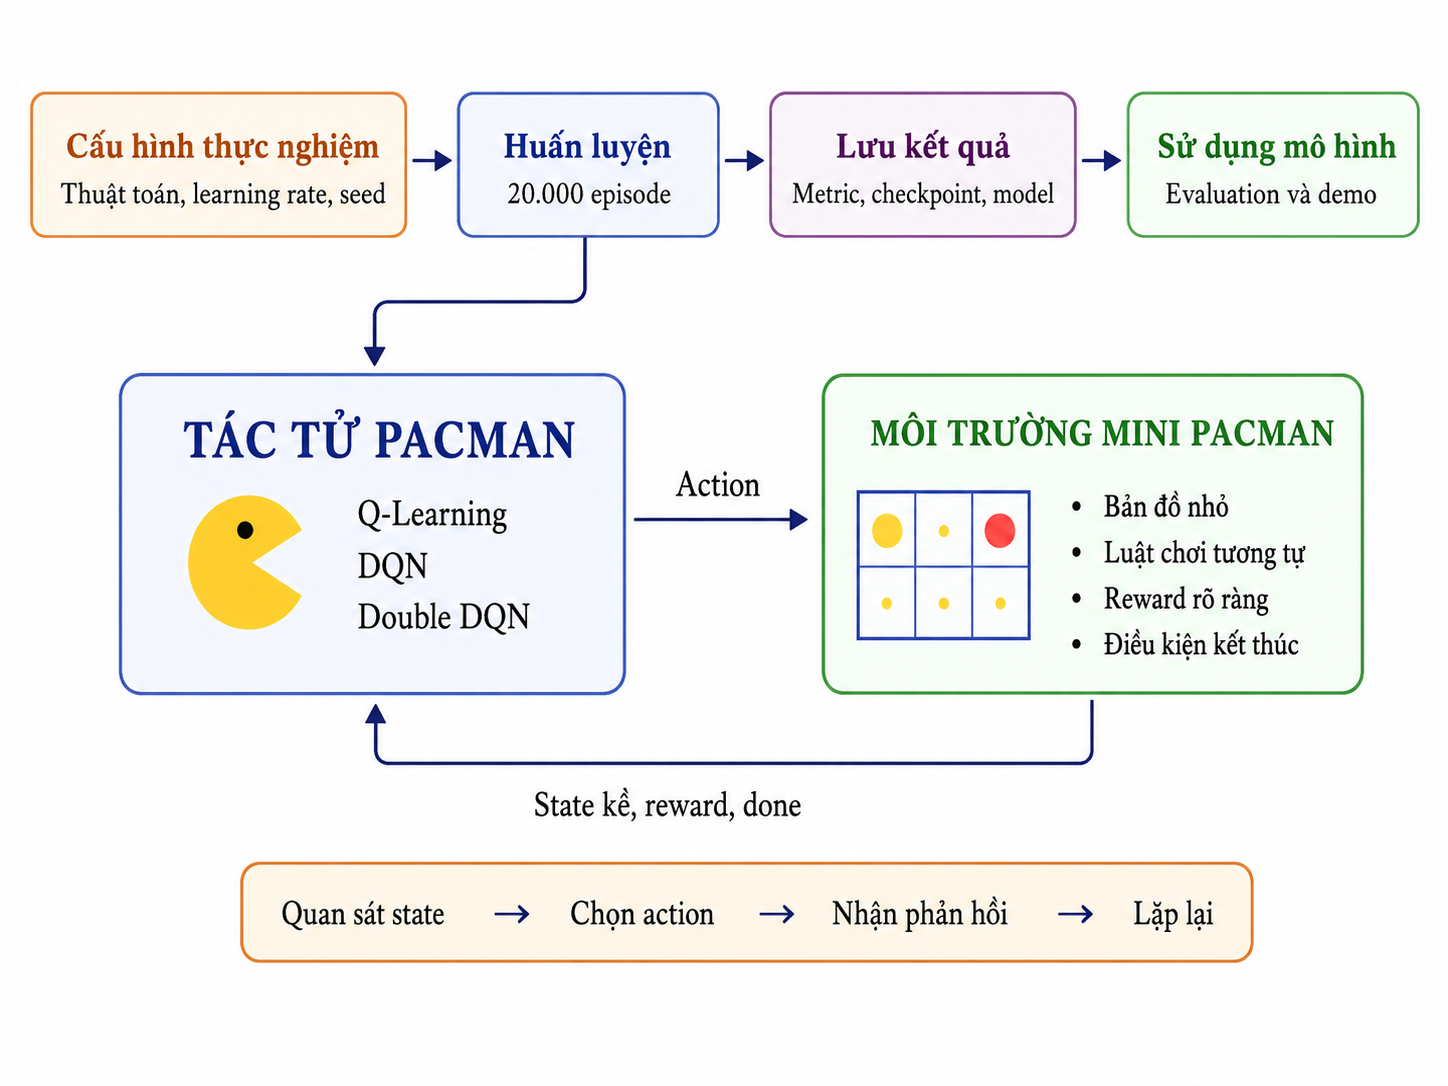
\includegraphics[width=0.94\textwidth]{image/hinh_3_1.png}
    \caption{Kiến trúc tổng thể của ứng dụng học tăng cường trong trò chơi Pacman.}
    \label{fig:system-overview}
\end{figure}

\subsection{Môi trường Mini Pacman}

Môi trường Mini Pacman tạo ra cùng một bài toán điều khiển cho cả ba phương pháp. Mỗi episode bắt đầu từ trạng thái khởi tạo của bản đồ. Sau khi nhận action, môi trường cập nhật trò chơi rồi trả về state kế tiếp, reward và cờ kết thúc. Tất cả thí nghiệm đều sử dụng bản đồ \texttt{medium}, ba mạng sống, ba ma và giới hạn 700 bước cho mỗi episode \cite{DRLPacmanGitHub}.

\subsubsection{Bản đồ và các thành phần trong môi trường}

Bản đồ \texttt{medium} có kích thước $15\times15$, gồm tường, hành lang, ghost door và khu vực xuất phát của ba ma ở trung tâm. Pacman xuất hiện ở phần dưới bản đồ. Hệ thống hành lang có nhiều ngã rẽ, buộc tác tử phải cân bằng giữa việc thu thập food, tránh ma và lựa chọn đường đi phù hợp.

Bản đồ chứa 62 food, trong đó bốn food gần các góc là power pellet. Ngoài ra, hai bonus fruit được đặt tại các vị trí cố định. Power pellet vẫn được tính vào tổng số food cần thu thập. Bonus fruit chỉ mang lại reward bổ sung và không ảnh hưởng đến điều kiện chiến thắng. \tabref{tab:map-components} tổng hợp các thành phần chính của môi trường.

\begin{table}[H]
    \centering
    \renewcommand{\arraystretch}{1.2}
    \small
    \begin{tabularx}{0.92\textwidth}{@{}
        >{\raggedright\arraybackslash}p{3.2cm}
        >{\centering\arraybackslash}p{2.1cm}
        >{\raggedright\arraybackslash}X
    @{}}
        \toprule
        \textbf{Thành phần} & \textbf{Số lượng} & \textbf{Vai trò trong môi trường} \\
        \midrule
        Bản đồ & $15\times15$ ô & Gồm tường, hành lang, ghost door và khu vực xuất phát của ma. \\
        Pacman & 1 & Tác tử được huấn luyện, bắt đầu với ba mạng sống. \\
        Ma & 3 & Blinky, Pinky và Inky, xuất phát tại khu vực trung tâm. \\
        Food & 62 & Phân bố trên hành lang và là điều kiện để hoàn thành bản đồ. \\
        Power pellet & 4 & Nằm trong 62 food và kích hoạt trạng thái frightened. \\
        Bonus fruit & 2 & Nằm ở vị trí cố định và cung cấp thêm reward. \\
        \bottomrule
    \end{tabularx}
    \caption{Các thành phần của bản đồ \texttt{medium} \cite{DRLPacmanGitHub}.}
    \label{tab:map-components}
\end{table}

\clearpage
\figref{fig:medium-map} minh họa trạng thái ban đầu của bản đồ trong một lượt demo. Bố cục bản đồ được giữ nguyên ở cả ba giai đoạn training, evaluation và demo.

\begin{figure}[H]
    \centering
    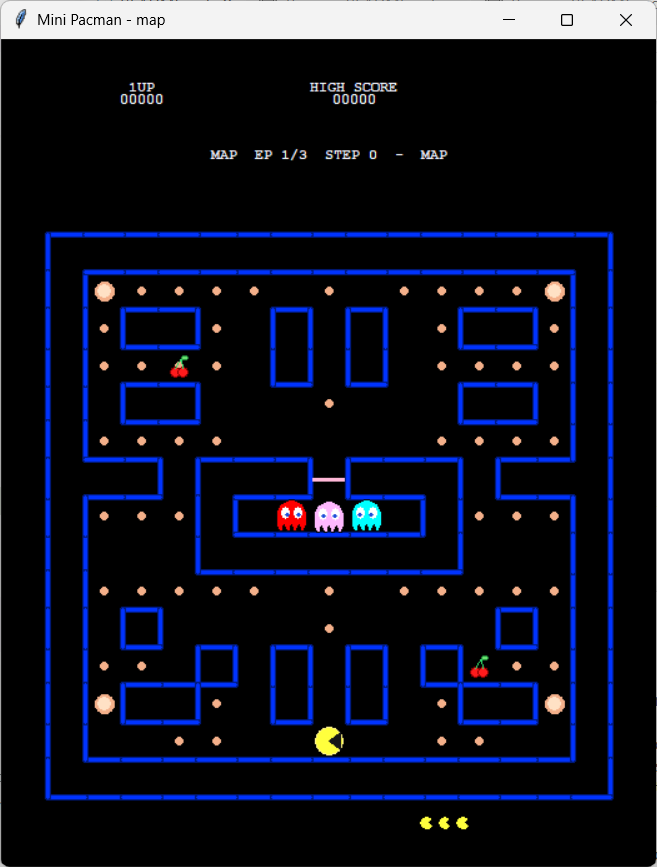
\includegraphics[width=0.49\textwidth]{image/demo_map.png}
    \caption{Bản đồ \texttt{medium} của môi trường Mini Pacman trong một lượt chạy demo.}
    \label{fig:medium-map}
\end{figure}

\subsubsection{Luật hoạt động và điều kiện kết thúc}

Trong mỗi environment step, Pacman di chuyển trước theo action đã chọn. Nếu hướng đi bị tường hoặc ghost door chặn, Pacman đứng tại chỗ và nhận penalty va tường. Sau đó, môi trường xử lý việc thu thập food, power pellet, bonus fruit và các va chạm tại vị trí mới. Ba ma tiếp tục thực hiện lượt di chuyển. Va chạm được kiểm tra thêm một lần trước khi môi trường trả về state mới, reward và cờ kết thúc.

Khi không frightened, ba ma luân phiên giữa scatter và chase. Mỗi ma sử dụng một mục tiêu riêng trong từng chế độ như trình bày trong \tabref{tab:ghost-targets}.

\begin{table}[H]
    \centering
    \renewcommand{\arraystretch}{1.14}
    \small
    \begin{tabularx}{0.96\textwidth}{@{}
        >{\raggedright\arraybackslash}p{2.5cm}
        >{\raggedright\arraybackslash}X
        >{\raggedright\arraybackslash}p{4.5cm}
    @{}}
        \toprule
        \textbf{Ma} &
        \makecell{\textbf{Mục tiêu trong}\\\textbf{chế độ chase}} &
        \makecell{\textbf{Mục tiêu trong}\\\textbf{chế độ scatter}} \\
        \midrule
        Blinky (đỏ) &
        Đuổi trực tiếp tới vị trí hiện tại của Pacman. &
        Góc trên bên phải của bản đồ, tại vị trí $(1,13)$. \\
        Pinky (hồng) &
        Nhắm tới điểm nằm trước Pacman tối đa bốn ô theo hướng di chuyển hiện tại để chặn đầu. &
        Góc trên bên trái của bản đồ, tại vị trí $(1,1)$. \\
        Inky (xanh lam) &
        Lấy điểm nằm trước Pacman tối đa hai ô, sau đó kéo dài vector từ Blinky tới điểm này thêm một lần để tạo mục tiêu. &
        Góc dưới bên phải của bản đồ, tại vị trí $(13,13)$. \\
        \bottomrule
    \end{tabularx}
    \caption{Mục tiêu di chuyển của ba ma trong chế độ chase và scatter \cite{DRLPacmanGitHub}.}
    \label{tab:ghost-targets}
\end{table}

Tại mỗi bước, ma loại hướng quay ngược nếu vẫn còn hướng hợp lệ khác, sau đó ưu tiên hướng tạo ra maze distance nhỏ nhất tới mục tiêu. Nếu nhiều hướng có cùng khoảng cách tốt nhất, hệ thống lựa chọn bằng bộ sinh số ngẫu nhiên đã được cố định seed. Cách xác định mục tiêu làm Blinky bám trực tiếp Pacman, Pinky tìm cách chặn đầu, còn Inky phối hợp vị trí của Blinky với hướng di chuyển của Pacman.

Power pellet đặt frightened timer bằng 35 bước. Trong thời gian này, ma chỉ di chuyển ở các environment step chẵn và ưu tiên hướng làm tăng maze distance tới Pacman. Nếu bị Pacman ăn, ma chuyển sang returning, quay về vị trí xuất phát rồi chờ bốn bước trước khi hoạt động trở lại. Các trạng thái chính và điều kiện chuyển đổi được minh họa trong \figref{fig:ghost-state-flow}.

\begin{figure}[H]
    \centering
    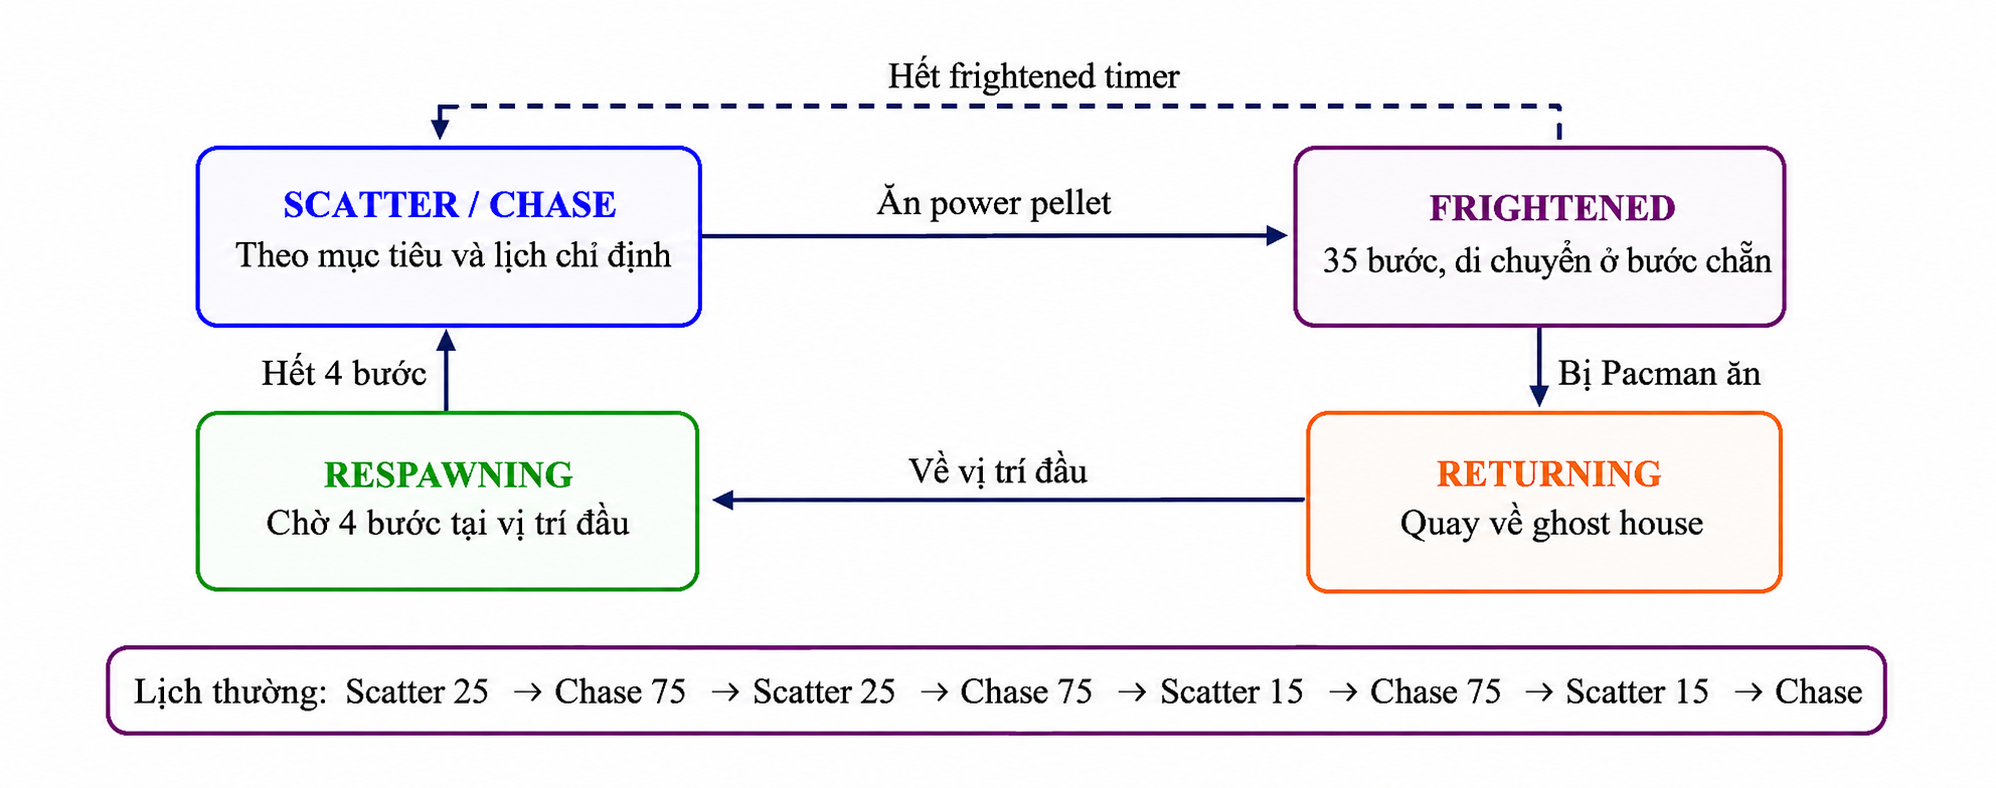
\includegraphics[width=0.94\textwidth]{image/hinh_3_3.png}
    \caption{Các trạng thái hoạt động và quá trình chuyển đổi của ma trong môi trường Mini Pacman.}
    \label{fig:ghost-state-flow}
\end{figure}

Episode kết thúc khi Pacman ăn hết 62 food, mất mạng cuối cùng hoặc đạt giới hạn 700 bước. Nếu Pacman bị bắt nhưng vẫn còn mạng, episode tiếp tục: Pacman và ba ma trở về vị trí xuất phát, còn food và bonus fruit đã ăn không được khôi phục. Do đó, tiến độ thu thập vật phẩm được giữ lại qua các lần mất mạng trong cùng một episode.

\subsection{Mô hình hóa bài toán học tăng cường}

Để lựa chọn action, tác tử cần nắm được vị trí của Pacman, vị trí và trạng thái của các ma, lượng food còn lại, số mạng và thời gian hiệu lực của power pellet. Môi trường mã hóa những thông tin này theo hai cách. Q-Learning sử dụng state dạng tuple, còn DQN và Double DQN nhận state dưới dạng vector số thực.

\subsubsection{Không gian và biểu diễn trạng thái}

State gốc gồm 17 giá trị, bao gồm hai tọa độ của Pacman, sáu tọa độ của ba ma, ba cờ returning, ba respawn timer, frightened timer, số mạng còn lại và một food mask. Q-Learning dùng trực tiếp tuple này làm khóa của Q-table. Mỗi khóa gắn với bốn Q-value tương ứng với bốn action. Các giá trị được khởi tạo bằng $0$ khi state xuất hiện lần đầu.

Đối với DQN và Double DQN, state được mở rộng thành vector 92 chiều. Food mask được tách thành 62 bit rồi ghép thêm thông tin về food gần nhất, ma đang hoạt động gần nhất, action hợp lệ và action nguy hiểm. Hai cách biểu diễn state được minh họa trong \figref{fig:state-representation}. Cấu trúc chi tiết của vector 92 chiều được trình bày trong \tabref{tab:state-vector}.

\begin{figure}[H]
    \centering
    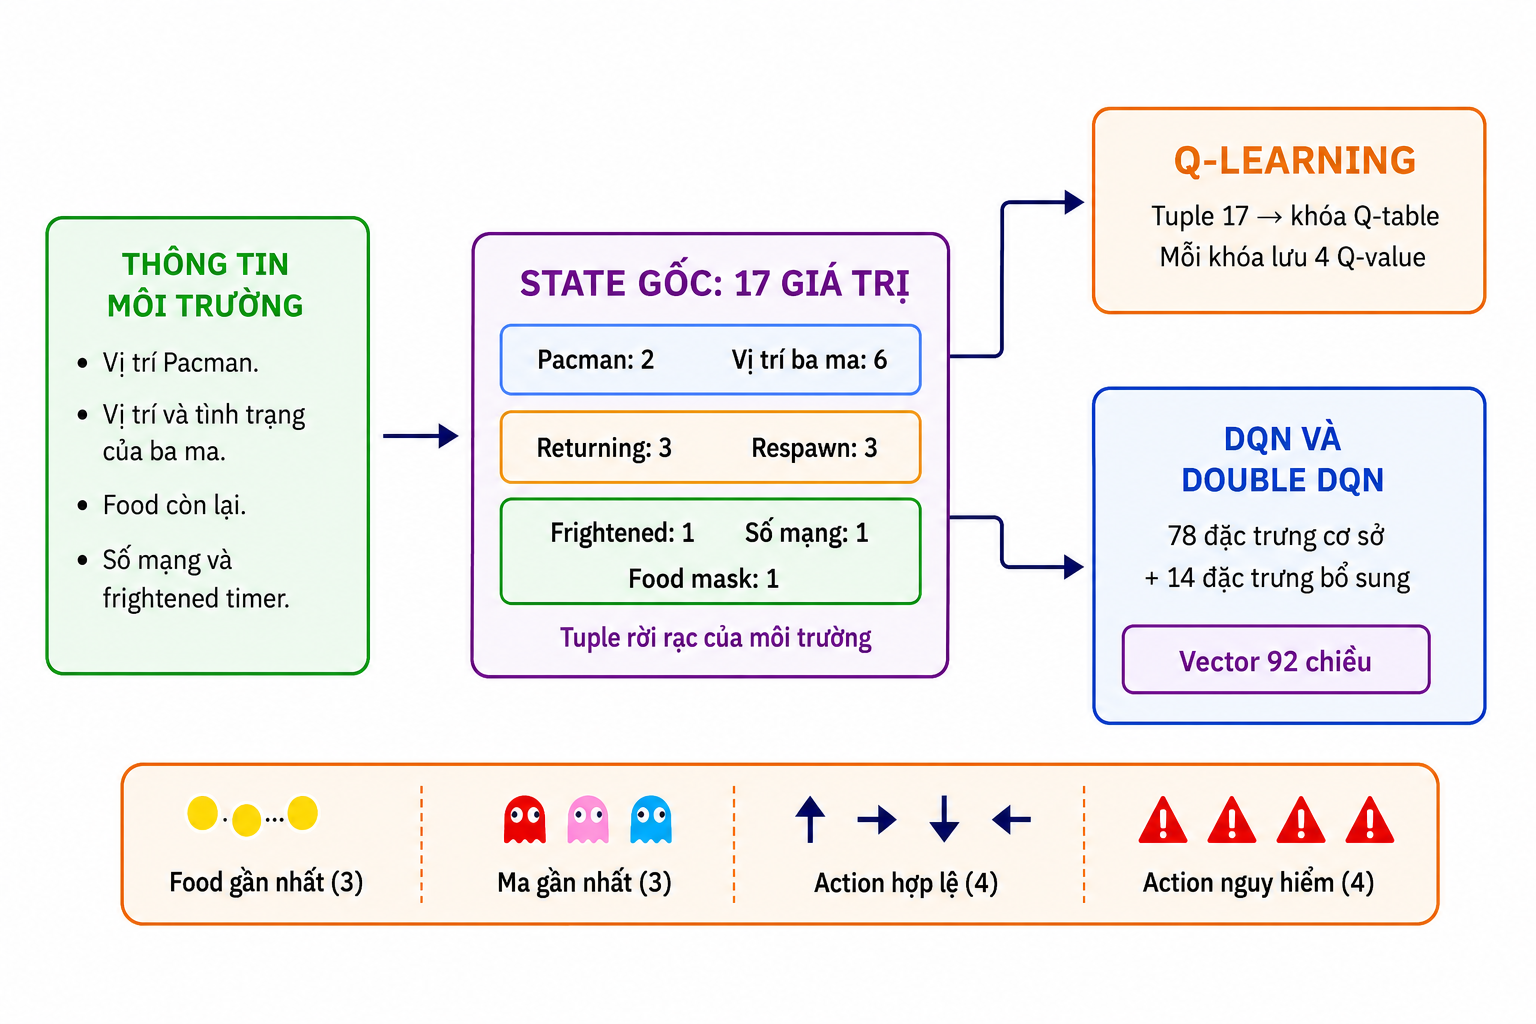
\includegraphics[width=0.94\textwidth]{image/hinh_3_4.png}
    \caption{Hai cách biểu diễn state được sử dụng cho Q-Learning và các phương pháp deep Q-learning.}
    \label{fig:state-representation}
\end{figure}

\begin{table}[H]
    \centering
    \renewcommand{\arraystretch}{1.16}
    \small
    \begin{tabularx}{0.96\textwidth}{@{}
        >{\raggedright\arraybackslash}p{3.7cm}
        >{\centering\arraybackslash}p{1.6cm}
        >{\raggedright\arraybackslash}X
    @{}}
        \toprule
        \textbf{Nhóm đặc trưng} & \textbf{Số chiều} & \textbf{Cách biểu diễn} \\
        \midrule
        Vị trí Pacman & 2 & Tọa độ hàng và cột, mỗi giá trị chia cho 14. \\
        Vị trí ba ma & 6 & Hai tọa độ cho mỗi ma, mỗi giá trị chia cho 14. \\
        Returning flags & 3 & Một cờ $0/1$ cho mỗi ma. \\
        Respawn timers & 3 & Một bộ đếm cho mỗi ma, chia cho 4. \\
        Số mạng còn lại & 1 & Số mạng chia cho 3. \\
        Frightened timer & 1 & Bộ đếm frightened chia cho 35. \\
        Food mask & 62 & Một cờ $0/1$ cho mỗi vị trí food cố định. \\
        Food gần nhất & 3 & Độ lệch hàng, độ lệch cột chia cho 14 và khoảng cách Manhattan chia cho 28. \\
        Ma đang hoạt động gần nhất & 3 & Độ lệch hàng, độ lệch cột chia cho 14 và khoảng cách Manhattan chia cho 28. \\
        Action hợp lệ & 4 & Bốn cờ $0/1$ theo thứ tự lên, phải, xuống và trái. \\
        Action nguy hiểm & 4 & Bốn cờ $0/1$, cho biết vị trí sau action có cách ma không quá hai ô Manhattan hay không. \\
        \midrule
        Tổng cộng & 92 & 78 đặc trưng cơ sở và 14 đặc trưng bổ sung. \\
        \bottomrule
    \end{tabularx}
    \caption{Cấu trúc vector state của DQN và Double DQN \cite{DRLPacmanGitHub}.}
    \label{tab:state-vector}
\end{table}

Food và ma gần nhất được lựa chọn theo maze distance, nhưng thành phần khoảng cách tương đối lưu trong vector là Manhattan distance. Khi xác định ma gần nhất, các ma đang returning hoặc respawning được loại bỏ. Nếu frightened timer lớn hơn $0$, bốn cờ action nguy hiểm đều bằng $0$. Power pellet không cần nhóm riêng vì bốn vị trí này cố định trong 62 food bit. Ảnh hưởng sau khi ăn được thể hiện qua frightened timer. Tường và ghost door cũng không được mã hóa thành toàn bộ bản đồ vì bố cục không thay đổi, trong khi bốn cờ action hợp lệ cung cấp thông tin di chuyển tại vị trí hiện tại \cite{DRLPacmanGitHub}.

Biểu diễn trên không chứa tình trạng của bonus fruit, số bước hiện tại, chế độ scatter/chase, action trước đó của Pacman và action trước đó của các ma. Các biến này vẫn tham gia vào luật chuyển trạng thái hoặc điều kiện kết thúc. Vì vậy, state được lựa chọn đáp ứng phạm vi thực nghiệm của đề tài nhưng không mô tả toàn bộ biến nội bộ của môi trường. Đầu vào của cả ba phương pháp được tạo từ dữ liệu trạng thái, không sử dụng ảnh chụp màn hình.

\subsubsection{Không gian hành động}

Không gian action gồm bốn hướng theo thứ tự lên, phải, xuống và trái. Tác tử không có action đứng yên. Cả Q-Learning, DQN và Double DQN đều có thể chọn một trong bốn action, kể cả khi hướng đó bị tường hoặc ghost door chặn. Trong trường hợp này, Pacman giữ nguyên vị trí và nhận penalty va tường. Bốn cờ action hợp lệ trong vector state chỉ cung cấp thông tin cho Q-network, không giới hạn trực tiếp action được chọn.

Trong training, action được chọn theo $\epsilon$-greedy. Ở exploration, tác tử chọn ngẫu nhiên một trong bốn action. Ở exploitation, action có Q-value lớn nhất được sử dụng. Trong evaluation, $\epsilon$ được đặt bằng $0$ để loại bỏ exploration.

\subsubsection{Thiết kế phần thưởng}

Reward vừa phản ánh kết quả của các sự kiện trong trò chơi, vừa định hướng Pacman thu thập food và duy trì khoảng cách an toàn với ma. Các thành phần có thể được cộng trong cùng một environment step. Chẳng hạn, khi Pacman ăn power pellet, reward của food và reward bổ sung của power pellet cùng được ghi nhận. Các giá trị chính xác được trình bày trong \tabref{tab:reward-design}.

\begin{table}[H]
    \centering
    % Compact this long table slightly so its caption stays clear of the footer.
    \renewcommand{\arraystretch}{1.05}
    \captionsetup{skip=5pt}
    \small
    \begin{tabularx}{0.92\textwidth}{@{}
        >{\raggedright\arraybackslash}X
        >{\centering\arraybackslash}p{2.6cm}
    @{}}
        \toprule
        \textbf{Thành phần reward} & \textbf{Giá trị cộng thêm} \\
        \midrule
        Mỗi environment step & $-0{,}10$ \\
        Va vào tường hoặc ghost door & $-1{,}00$ \\
        Ăn một food & $+10{,}00$ \\
        Food là power pellet & $+50{,}00$ \\
        Ăn một bonus fruit & $+100{,}00$ \\
        Ăn một ma đang frightened & $+200{,}00$ \\
        Ăn hết food và thắng episode & $+100{,}00$ \\
        Bị ma bắt và mất một mạng & $-50{,}00$ \\
        Không thắng và không bị ma bắt trong bước hiện tại & $+0{,}02$ \\
        Tiến gần food gần nhất khi chưa ăn vật phẩm & $+0{,}03$ \\
        Đi xa food gần nhất khi chưa ăn vật phẩm & $-0{,}03$ \\
        Tăng khoảng cách tới ma gần nhất & $+0{,}05$ \\
        Tiến gần ma trong vùng nguy hiểm không quá năm ô & $-0{,}10$ \\
        Chạm giới hạn 700 bước & $-10{,}00$ \\
        \bottomrule
    \end{tabularx}
    \caption{Các thành phần reward của môi trường Mini Pacman \cite{DRLPacmanGitHub}.}
    \label{tab:reward-design}
\end{table}

Reward tiến gần hoặc đi xa food chỉ được áp dụng khi Pacman không ăn food hay bonus fruit ở bước hiện tại và trên bản đồ vẫn còn food. Reward tồn tại được cộng sau khi kiểm tra điều kiện thắng và bị bắt, nhưng trước khi kiểm tra giới hạn 700 bước. Vì vậy, bước chạm giới hạn vẫn có thể nhận $+0{,}02$ trước khi nhận penalty timeout. Các thành phần reward dựa trên khoảng cách tới food và ma sử dụng maze distance. Riêng cờ action nguy hiểm trong vector state sử dụng Manhattan distance sau khi thử action.

\subsection{Cài đặt các thuật toán}

Cả ba phương pháp đều nhận cùng loại phản hồi từ môi trường nhưng khác nhau ở cơ chế học. Q-Learning cập nhật trực tiếp Q-table sau mỗi transition. DQN và Double DQN đưa transition vào replay buffer rồi lấy mẫu theo mini-batch để cập nhật Q-network \cite{DRLPacmanGitHub}.

\subsubsection{Q-Learning}

Nguyên lý lựa chọn action và cập nhật Q-table đã được trình bày tại Mục 2.2, đồng thời được minh họa trong \figref{fig:q-learning-principle}. Khi áp dụng vào Mini Pacman, tuple state gồm 17 giá trị được dùng làm khóa của Q-table. Mỗi khóa lưu bốn Q-value tương ứng với bốn action. Sau mỗi transition, Q-value của cặp state--action vừa thực hiện được cập nhật theo phương trình~\eqref{eq:q-learning-update}. Nếu transition kết thúc episode, thành phần bootstrap bằng $0$. Ngược lại, target sử dụng Q-value lớn nhất của state kế tiếp.

Q-Learning lựa chọn action theo chiến lược $\epsilon$-greedy và giảm epsilon sau mỗi episode. Tại từng mốc checkpoint, hệ thống lưu Q-table, epsilon, trạng thái của bộ sinh số ngẫu nhiên và tiến độ huấn luyện. Nhờ đó, thí nghiệm có thể tiếp tục từ mốc gần nhất nếu bị gián đoạn. Mô hình cuối chỉ chứa Q-table đã học để phục vụ evaluation và demo.

\subsubsection{DQN}

DQN sử dụng mạng multilayer perceptron với đầu vào là vector state 92 chiều và đầu ra là bốn Q-value. Mạng có hai hidden layer, mỗi layer gồm 128 neuron và sử dụng hàm kích hoạt ReLU. Output layer không dùng hàm kích hoạt. Online network và target network có cùng kiến trúc, mỗi mạng gồm 28.932 tham số. Cấu trúc mạng và mối quan hệ giữa hai nhánh được minh họa trong \figref{fig:q-network-architecture}.

\begin{figure}[H]
    \centering
    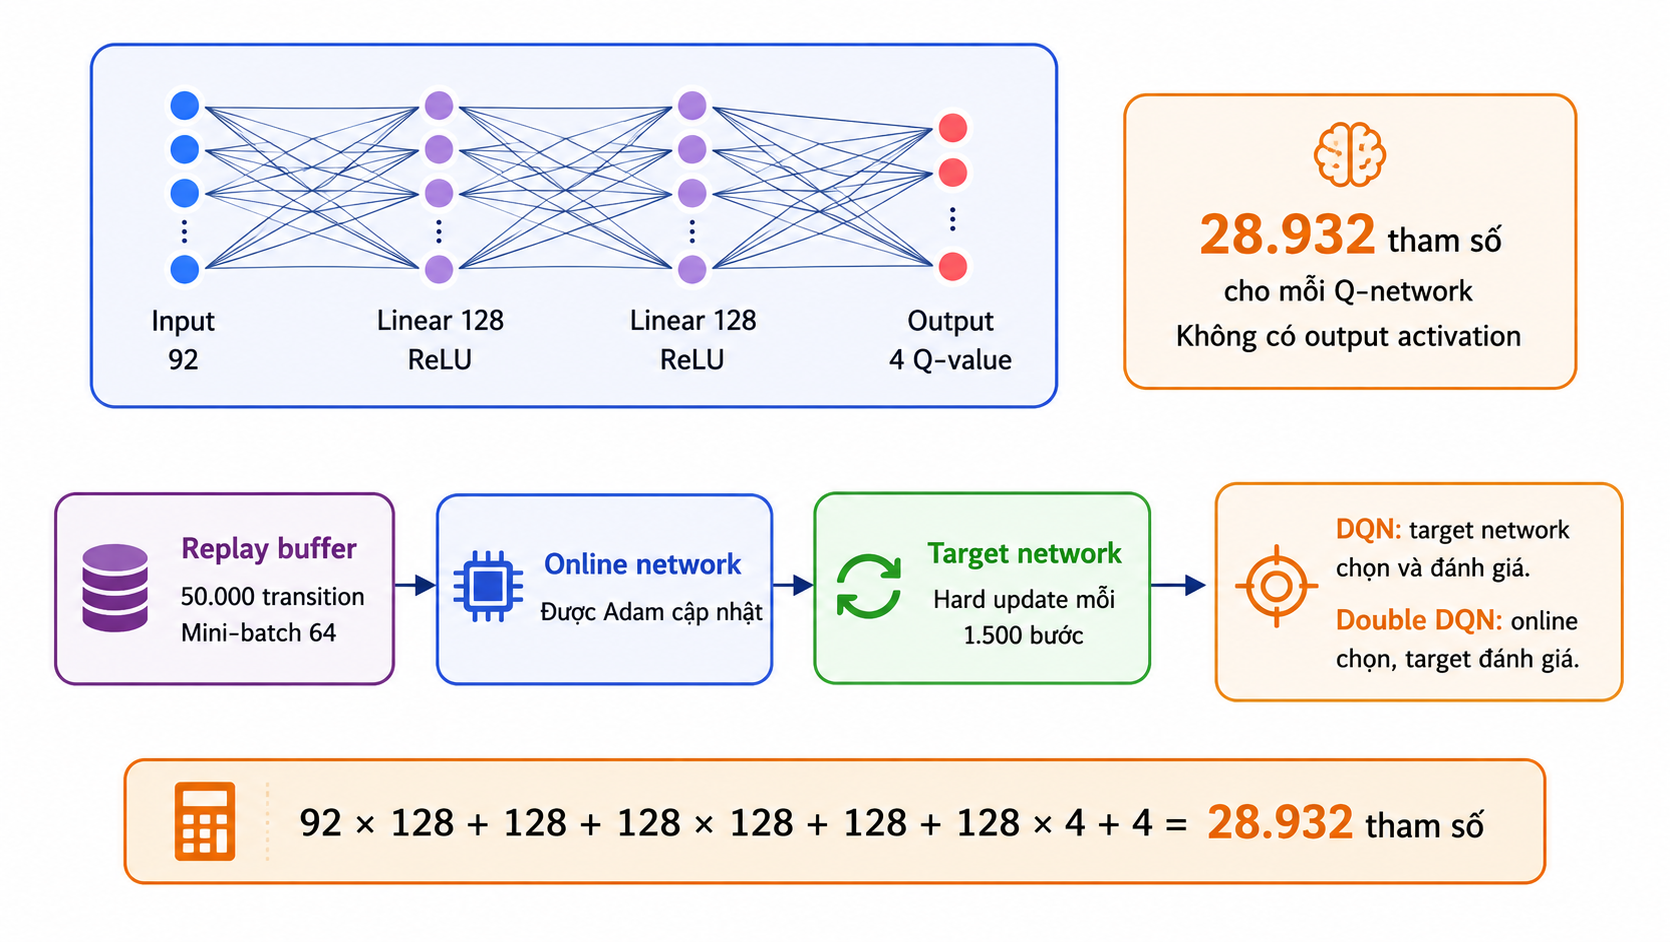
\includegraphics[width=0.94\textwidth]{image/hinh_3_5.png}
    \caption{Kiến trúc Q-network và vai trò của online network, target network trong hai phương pháp.}
    \label{fig:q-network-architecture}
\end{figure}

Mỗi transition gồm state vector, action, reward, next-state vector và cờ kết thúc. Các transition được lưu trong replay buffer hoạt động theo cơ chế FIFO với sức chứa 50.000 mẫu. Việc học bắt đầu sau khi tác tử tích lũy đủ 10.000 environment step. Ở mỗi lần cập nhật, hệ thống lấy ngẫu nhiên 64 transition không lặp trong cùng mini-batch để tối ưu online network. Sau mỗi 1.500 environment step, toàn bộ trọng số của online network được sao chép sang target network.

Online network được tối ưu bằng Adam với learning rate tương ứng của từng cấu hình. Hàm \texttt{SmoothL1Loss} được áp dụng cho TD error, còn gradient norm được giới hạn ở $10{,}0$. DQN target được tính theo phương trình~\eqref{eq:dqn-target}. Epsilon chỉ giảm sau khi online network thực hiện một lần cập nhật thành công. Vì vậy, epsilon được giữ nguyên trong 10.000 bước thu thập dữ liệu ban đầu.

Mô hình cuối chỉ lưu state dictionary của online network. Khi mô hình được tải để evaluation hoặc demo, target network được đồng bộ lại từ online network. Trong khi đó, checkpoint phục vụ việc tiếp tục training nên lưu thêm target network, optimizer, replay buffer, epsilon, trạng thái bộ sinh số ngẫu nhiên và tiến độ huấn luyện.

\subsubsection{Double DQN}

Double DQN giữ nguyên vector đầu vào, kiến trúc mạng, optimizer, loss, replay buffer, chiến lược exploration và lịch cập nhật target network của DQN. Điểm khác biệt duy nhất là cách tính target cho next state. Online network chọn action theo phương trình~\eqref{eq:ddqn-action-selection}. Sau đó, target network đánh giá action đã chọn theo phương trình~\eqref{eq:ddqn-target}. TD error vẫn được tối ưu bằng \texttt{SmoothL1Loss}, nhưng DQN target được thay bằng Double DQN target. Các siêu tham số còn lại được giữ giống DQN tại cùng learning rate.

\subsection{Thiết kế thực nghiệm}

Thực nghiệm gồm chín cấu hình, được tạo từ ba thuật toán và ba giá trị learning rate. Trong phạm vi từng thuật toán, chỉ learning rate được thay đổi. Bản đồ, số episode, seed, lịch evaluation và những thiết lập còn lại được giữ cố định. Cách bố trí này giúp đánh giá ảnh hưởng của learning rate mà không làm thay đổi đồng thời các yếu tố khác.

\subsubsection{Cấu hình và siêu tham số}

Ba giá trị learning rate được khảo sát là $0{,}0001$, $0{,}0005$ và $0{,}001$. Trong Q-Learning, tham số này điều khiển trực tiếp mức cập nhật của Q-table. Với DQN và Double DQN, learning rate thuộc optimizer Adam. Do hai cơ chế học khác nhau, kết quả chỉ được so sánh giữa các learning rate trong cùng một thuật toán. Một giá trị giống nhau không có nghĩa là Q-table và Q-network thay đổi với mức độ tương đương.

\begin{itemize}
    \item \textbf{Thiết bị huấn luyện:} laptop cá nhân MSI Cyborg 15, trang bị GPU NVIDIA GeForce RTX 4050 Laptop GPU với 6 GB VRAM.
\end{itemize}

Các tham số chung của chín thí nghiệm được trình bày trong \tabref{tab:common-hyperparameters}.

\begin{table}[H]
    \centering
    \renewcommand{\arraystretch}{1.18}
    \small
    \begin{tabularx}{0.88\textwidth}{@{}
        >{\raggedright\arraybackslash}X
        >{\centering\arraybackslash}p{4.4cm}
    @{}}
        \toprule
        \textbf{Tham số} & \textbf{Giá trị} \\
        \midrule
        Learning rate & $0{,}0001$, $0{,}0005$ và $0{,}001$ \\
        Số episode training & 20.000 \\
        Discount factor & $0{,}99$ \\
        Layout & \texttt{medium}, $15\times15$ ô \\
        Số bước tối đa mỗi episode & 700 \\
        Số mạng sống & 3 \\
        Số ma & 3 \\
        Training seed & 42 \\
        Checkpoint interval & 1.000 episode \\
        Evaluation interval & 1.000 episode \\
        Số episode mỗi lần evaluation & 20 \\
        Evaluation seed & 10042 \\
        \bottomrule
    \end{tabularx}
    \caption{Các tham số chung của chín cấu hình thực nghiệm \cite{DRLPacmanGitHub}.}
    \label{tab:common-hyperparameters}
\end{table}

Các thiết lập riêng của từng phương pháp được tổng hợp trong \tabref{tab:algorithm-hyperparameters}. DQN và Double DQN dùng cùng cấu hình. Sự khác biệt giữa chúng nằm ở cách tính target.

\begin{table}[H]
    \centering
    \renewcommand{\arraystretch}{1.15}
    \footnotesize
    \begin{tabularx}{\textwidth}{@{}
        >{\raggedright\arraybackslash}p{3.5cm}
        >{\centering\arraybackslash}p{3.2cm}
        >{\centering\arraybackslash}X
        >{\centering\arraybackslash}X
    @{}}
        \toprule
        \textbf{Tham số} & \textbf{Q-Learning} & \textbf{DQN} & \textbf{Double DQN} \\
        \midrule
        Epsilon ban đầu & $1{,}0$ & $1{,}0$ & $1{,}0$ \\
        Epsilon nhỏ nhất & $0{,}05$ & $0{,}02$ & $0{,}02$ \\
        Epsilon decay & $0{,}99985$/episode & $0{,}999997$/update & $0{,}999997$/update \\
        Kích thước hidden layer & Không sử dụng & 128, 128 & 128, 128 \\
        Batch size & Không sử dụng & 64 & 64 \\
        Replay capacity & Không sử dụng & 50.000 & 50.000 \\
        Learning starts & Không sử dụng & 10.000 bước & 10.000 bước \\
        Target update interval & Không sử dụng & 1.500 bước & 1.500 bước \\
        Optimizer & Không sử dụng & Adam & Adam \\
        Loss & Không sử dụng & SmoothL1 & SmoothL1 \\
        Gradient clipping & Không sử dụng & Max norm $10{,}0$ & Max norm $10{,}0$ \\
        \bottomrule
    \end{tabularx}
    \caption{Các tham số riêng của Q-Learning, DQN và Double DQN \cite{DRLPacmanGitHub}.}
    \label{tab:algorithm-hyperparameters}
\end{table}

Training seed, evaluation seed và cấu hình của từng thí nghiệm được giữ cố định để hỗ trợ tái lập kết quả.

\subsubsection{Quy trình huấn luyện và đánh giá}

Mỗi thí nghiệm bắt đầu bằng việc khởi tạo môi trường và tác tử theo cấu hình tương ứng. Trong từng episode, tác tử liên tục tương tác với môi trường để cập nhật Q-table hoặc Q-network. Các metric training được ghi lại sau mỗi episode. Cứ 1.000 episode, hệ thống lưu checkpoint và thực hiện một lần evaluation độc lập. Quy trình đầy đủ được tóm tắt trong \figref{fig:experiment-process}.

\begin{figure}[H]
    \centering
    \resizebox{0.94\textwidth}{!}{%
    \begin{tikzpicture}[x=1cm,y=1cm,font=\fontsize{8.5}{10.2}\selectfont]
            \node[chthreeorange, minimum width=10.5cm, minimum height=0.75cm] at (7.6,4.35)
                {9 thí nghiệm $=$ 3 thuật toán $\times$ 3 learning rate: $0{,}0001$, $0{,}0005$, $0{,}001$};
    
            \foreach \x/\n/\col in {1.25/1/orange,4.35/2/blue,7.45/3/violet,10.55/4/green,13.65/5/orange}{
                \fill[\col!72] (\x,3.25) circle (0.30);
                \node[font=\bfseries,text=white] at (\x,3.25) {\n};
            }
            \draw[chthreeflow] (1.58,3.25) -- (4.02,3.25);
            \draw[chthreeflow] (4.68,3.25) -- (7.12,3.25);
            \draw[chthreeflow] (7.78,3.25) -- (10.22,3.25);
            \draw[chthreeflow] (10.88,3.25) -- (13.32,3.25);
    
            \node[chthreeorange, minimum width=2.6cm, minimum height=1.65cm] at (1.25,1.8)
                {\textbf{Khởi tạo}\\Layout medium\\Training seed 42};
            \node[chthreeblue, minimum width=2.6cm, minimum height=1.65cm] at (4.35,1.8)
                {\textbf{Training}\\20.000 episode\\$\epsilon$-greedy};
            \node[chthreepurple, minimum width=2.6cm, minimum height=1.65cm] at (7.45,1.8)
                {\textbf{Mỗi 1.000 episode}\\Lưu checkpoint\\Chạy evaluation};
            \node[chthreegreen, minimum width=2.6cm, minimum height=1.65cm] at (10.55,1.8)
                {\textbf{Evaluation}\\20 episode\\$\epsilon=0$, seed 10042};
            \node[chthreeorange, minimum width=2.6cm, minimum height=1.65cm] at (13.65,1.8)
                {\textbf{Hoàn tất}\\Lưu model cuối\\Ghi nhận metric};
    
            \node[chthreepurple, minimum width=10.2cm, minimum height=0.65cm] at (7.6,0.35)
                {Evaluation không cập nhật Q-table, replay buffer, optimizer hoặc tham số network.};
        \end{tikzpicture}
    }
    \caption{Quy trình training, lưu checkpoint, evaluation và lưu mô hình cuối.}
    \label{fig:experiment-process}
\end{figure}

Trong mỗi lần evaluation, $\epsilon$ được đặt bằng $0$ và tác tử chạy 20 episode với evaluation seed 10042. Tác tử chỉ sử dụng cơ chế chọn action của policy hiện tại. Q-table, replay buffer, optimizer và tham số mạng đều không được cập nhật. Sau 20.000 episode training, hệ thống lưu mô hình cuối cùng và ghi nhận kết quả của lần evaluation cuối.

Checkpoint và final model phục vụ hai mục đích khác nhau. Checkpoint lưu các thành phần cần thiết để tiếp tục training từ mốc gần nhất. Final model chỉ giữ Q-table đối với Q-Learning hoặc trọng số online network đối với DQN và Double DQN, phù hợp cho evaluation và demo.

\subsubsection{Tiêu chí đánh giá}

Mỗi lần evaluation gồm 20 episode với $\epsilon=0$. Thiết lập này giúp kết quả phản ánh trực tiếp policy đã học mà không bị ảnh hưởng bởi hành động thăm dò. Gọi $N=20$ là số episode trong một lần evaluation. Ở episode thứ $i$, $R_i$, $T_i$ và $F_i$ lần lượt biểu thị reward tích lũy, số bước thực hiện và số food đã ăn. Các tiêu chí đánh giá được xây dựng từ ba đại lượng này.

\noindent\textbf{Reward trung bình.}
\begin{equation}
    \overline{R}=\frac{1}{N}\sum_{i=1}^{N}R_i.
    \label{eq:average-reward}
\end{equation}
Đại lượng $\overline{R}$ phản ánh reward tích lũy trung bình của tác tử. Do reward có thể được cộng từ nhiều sự kiện trong cùng một bước, chỉ số này cần được đọc cùng win rate, completion rate và số bước trung bình thay vì dùng riêng để kết luận về chất lượng policy.

\noindent\textbf{Số bước trung bình.}
\begin{equation}
    \overline{T}=\frac{1}{N}\sum_{i=1}^{N}T_i.
    \label{eq:average-steps}
\end{equation}
$\overline{T}$ cho biết độ dài trung bình của một episode trước khi tác tử chiến thắng, mất mạng cuối cùng hoặc đạt giới hạn bước. Số bước lớn không đồng nghĩa với policy tốt hơn nên chỉ số này phải được xem cùng win rate và completion rate.

\noindent\textbf{Số food ăn được trung bình.}
\begin{equation}
    \overline{F}=\frac{1}{N}\sum_{i=1}^{N}F_i.
    \label{eq:average-food}
\end{equation}
$\overline{F}$ biểu thị lượng food trung bình tác tử thu thập được trong một episode, qua đó cho thấy mức tiến triển của tác tử trên bản đồ.

\noindent\textbf{Completion rate trung bình.}
\begin{equation}
    \overline{C}=\frac{1}{N}\sum_{i=1}^{N}\left(\frac{F_i}{62}\times100\%\right).
    \label{eq:average-completion}
\end{equation}
Mỗi episode có tổng cộng 62 food. Vì vậy, $F_i/62$ là tỷ lệ bản đồ được hoàn thành trong episode thứ $i$, còn $\overline{C}$ là tỷ lệ hoàn thành trung bình của toàn bộ 20 episode.

\noindent\textbf{Win rate.}
\begin{equation}
    \mathrm{WinRate}=\frac{1}{N}\sum_{i=1}^{N}\mathbf{1}(F_i=62)\times100\%.
    \label{eq:evaluation-win-rate}
\end{equation}
Hàm chỉ thị $\mathbf{1}(F_i=62)$ nhận giá trị $1$ khi tác tử ăn hết 62 food và chiến thắng, ngược lại nhận giá trị $0$. Win rate trong evaluation được tính độc lập trên 20 episode tại từng mốc. Chỉ số này khác với win rate tích lũy trong lịch sử training.

\noindent\textbf{Reward tốt nhất.}
\begin{equation}
    R_{\max}=\max_{1\leq i\leq N}R_i.
    \label{eq:best-reward}
\end{equation}
$R_{\max}$ ghi nhận reward tích lũy lớn nhất trong 20 episode, thể hiện kết quả tốt nhất mà policy đạt được ở lần evaluation đó.

\noindent\textbf{Completion rate tốt nhất.}
\begin{equation}
    C_{\max}=\max_{1\leq i\leq N}\left(\frac{F_i}{62}\times100\%\right).
    \label{eq:best-completion}
\end{equation}
$C_{\max}$ là tỷ lệ hoàn thành lớn nhất trong 20 episode, cho biết policy đã tiến gần đến việc hoàn thành bản đồ nhất ở mức nào.

Đối với DQN và Double DQN, loss được tính bằng \texttt{SmoothL1Loss} theo phương trình~\eqref{eq:dqn-loss}. Q-Learning không sử dụng chỉ số này vì không huấn luyện mạng nơ-ron. Hệ thống còn thống kê số episode kết thúc do chiến thắng, mất mạng cuối cùng hoặc đạt giới hạn bước. \tabref{tab:evaluation-metrics} tóm tắt toàn bộ tiêu chí được sử dụng.

\begin{table}[H]
    \centering
    \renewcommand{\arraystretch}{1.08}
    \captionsetup{skip=5pt}
    \small
    \begin{tabularx}{0.96\textwidth}{@{}
        >{\raggedright\arraybackslash}p{3.4cm}
        >{\raggedright\arraybackslash}X
    @{}}
        \toprule
        \textbf{Metric} & \textbf{Ý nghĩa và cách tính} \\
        \midrule
        Average reward & Reward tích lũy trung bình của 20 episode evaluation, được đọc cùng win rate, completion rate và số bước. \\
        Average steps & Số bước trung bình trước khi episode kết thúc, được đọc cùng win rate và completion rate. \\
        Average food eaten & Số food được ăn trung bình trong 20 episode. \\
        Average completion rate & Trung bình tỷ lệ food đã ăn trên tổng số 62 food của từng episode. \\
        Win rate & Số episode chiến thắng chia cho 20 episode evaluation. \\
        Loss & Trung bình \texttt{SmoothL1Loss} của các update trong một episode training, chỉ có ở DQN và Double DQN. \\
        Best reward & Reward lớn nhất trong 20 episode evaluation. \\
        Best completion rate & Completion rate lớn nhất trong 20 episode evaluation. \\
        Wins, caught, timeout & Số episode kết thúc do thắng, mất mạng cuối cùng hoặc đạt giới hạn bước. \\
        \bottomrule
    \end{tabularx}
    \caption{Các tiêu chí được sử dụng để đánh giá kết quả thực nghiệm.}
    \label{tab:evaluation-metrics}
\end{table}

Lần đánh giá cuối sử dụng $\epsilon=0$ nên phản ánh policy đã học mà không trộn lẫn exploration.
